\documentclass{beamer}
\usepackage[spanish]{babel}
\usepackage{tikz} 
\usepackage{tikz-network}
\usepackage[utf8]{inputenc}
\usepackage{algorithm,algorithmic}
\graphicspath{{imagenes/}{../imagenes/}}
\usetheme{CambridgeUS}
\title{Minimum cost flows}
\author{Lic. Eder Ismael Alanís Fernández\\ Lic. Arnoldo Del Toro Peña }
\institute{Universidad Autónoma de Nuevo León}
\begin{document}

\begin{frame}
 \titlepage
\end{frame}

\begin{frame}
 \frametitle{Assumptions}
\begin{block}<1->{Assumption 1}
All data are integral.
\end{block}

\begin{block}<2->{Assumption 2}
The network are directed.
\end{block}

\begin{block}<3->{Assumption 3}
  Se satisface la ecuación: $$\sum_{i \in N} {b(i)} = 0$$.
  \end{block}
\end{frame}

\begin{frame}
  \begin{block}<1->{Assumption 4}
    We assume that the network G contains an uncapacitated
    directed path.
  \end{block}
  \begin{block}<2->{Assumption 5}
    All arc costs are nonnegative.
  \end{block}
    
\end{frame}

\begin{frame}
\frametitle{Aplications}
\framesubtitle{Dsitribution problems}
\begin{figure}[h!t]
\centering
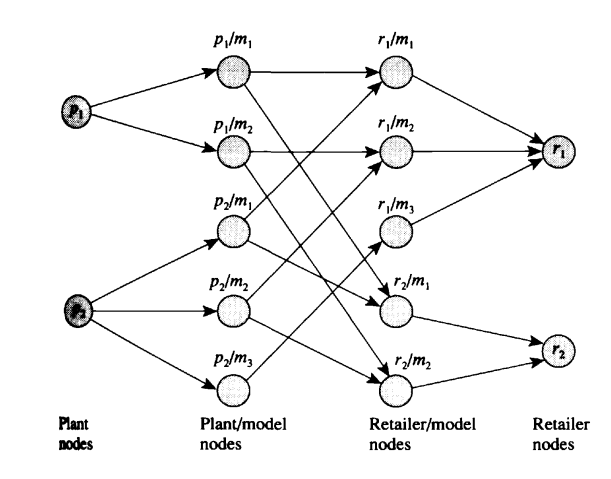
\includegraphics[scale = 0.4 ]{distributionproblem.png}
%\caption{}
%\label{}
\end{figure}
\end{frame}

\begin{frame}
  \frametitle{Aplications}
  \framesubtitle{Reconstruoting the Left Ventriole from
  X-ray Projections}
  \begin{figure}[h!t]
  \centering
  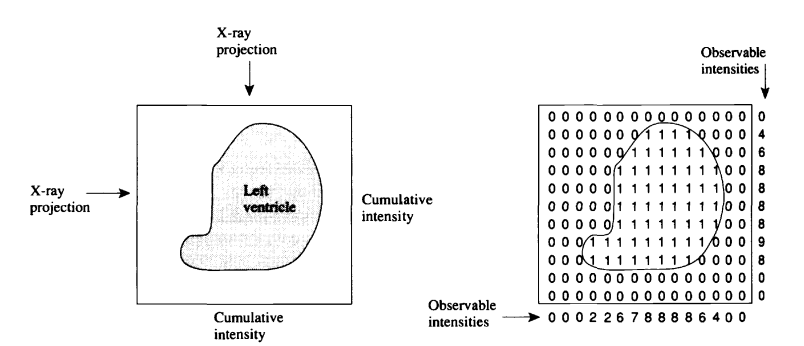
\includegraphics[scale = 0.4 ]{x-rayproblem.png}
  %\caption{}
  %\label{}
  \end{figure}
  \end{frame}

\begin{frame}
  \frametitle{Aplications}
  \framesubtitle{Racial balancing of schools}
  \begin{figure}[h!t]
  \centering
  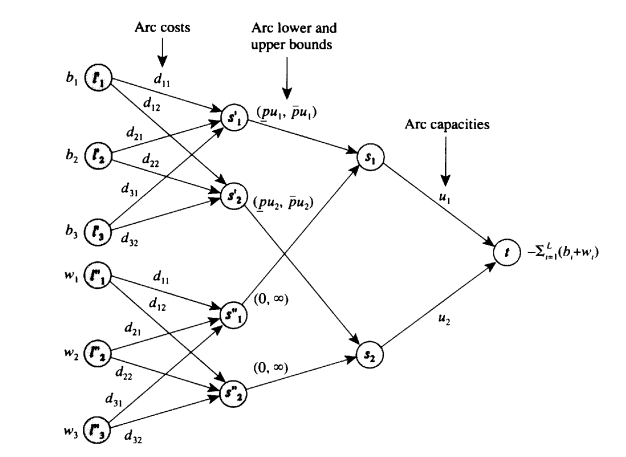
\includegraphics[scale = 0.4 ]{scholarproblem.png}
  %\caption{}
  %\label{}
  \end{figure}
\end{frame}

\begin{frame}
  \frametitle{Aplications}
  \framesubtitle{Optimal Loading of a Hopping
  Airplane}
  \begin{figure}[h!t]
  \centering
  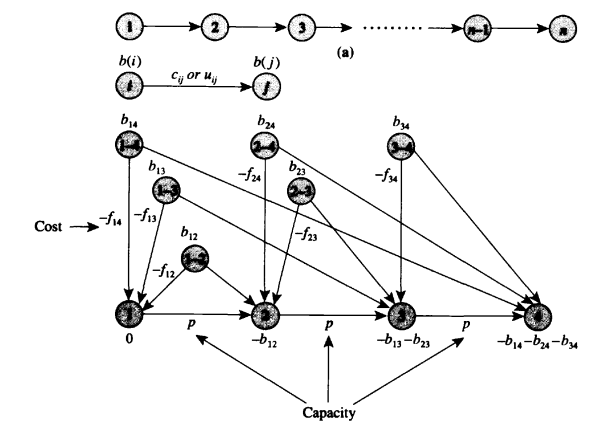
\includegraphics[scale = 0.4 ]{airplaneproblem.png}
  %\caption{}
  %\label{}
  \end{figure}
\end{frame}

\begin{frame}
  \frametitle{Aplications}
  \framesubtitle{Scheduling with Deferral Costs}
\begin{figure}[h!t]
\centering
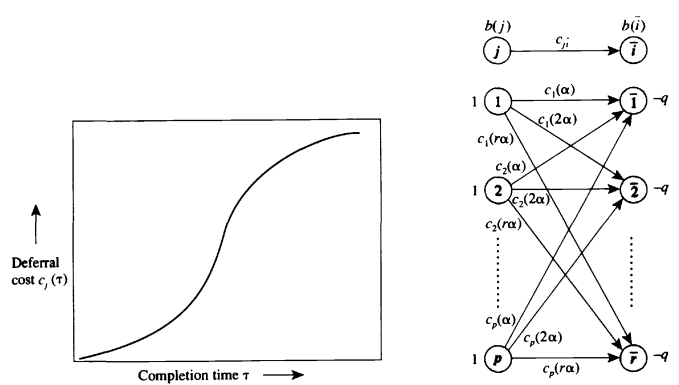
\includegraphics[scale = 0.4 ]{deferralproblem.png}
%\caption{}
%\label{}
\end{figure}  
\end{frame}

\begin{frame}
  \frametitle{Aplications}
  \framesubtitle{Linear Programs with Consecutive 1 's
  in Columns}
  \begin{figure}[h!t]
  \centering
  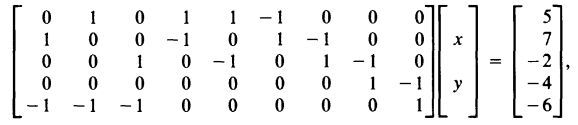
\includegraphics[scale = 0.5 ]{matrizlinearproblem.png}
  %\caption{}
  %\label{}
  \end{figure}
\end{frame}

\begin{frame}
  \frametitle{Aplications}
  \framesubtitle{Linear Programs with Consecutive 1 's
  in Columns}
  \begin{figure}[h!t]
  \centering
  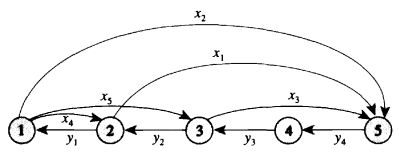
\includegraphics[scale = 0.8 ]{linearproblem.png}
  %\caption{}
  %\label{}
  \end{figure}
\end{frame}

\begin{frame}
  \frametitle{Aplications}
  \framesubtitle{General}
  
  \begin{enumerate}
  \item Optimal capacity scheduling.
  \item Employment schudeling.
  \item Equipment replacement.
  \end{enumerate}
\end{frame}

\begin{frame}{Optimality conditions}{Negative Cycle Optimality Conditions}

\begin{block}{Theorem: }
  A feasible solution x* is
  an optimal solution of the minimum cost flow problem if and only if it satisfies the
  negative cycle optimality conditions: namely, the residual network G(x*) contains
  no negative cost (directed) cycle.
\end{block}
\end{frame}

\begin{frame}{Optimality conditions}{Reduced Cost Optimality Conditions}

  \begin{block}{Notas: }
  $\pi(i)$ as the potential of node i, is the linear programming dual variable corresponding to the mass balance constraint of node i. \\
  Reduced cost of any arc as: $$c_{ij}^{\pi} = c_{ij} - \pi(i) + \pi(j)$$ \\
  Property: \\ 
  \begin{enumerate}
    \item For any directed path P from node k to node I, $\displaystyle \sum_{(i,j) \in P} c_{ij}^{\pi} = \sum_{(i,j) \in P} c_{ij} - \pi(k)+\pi(l)$
    \item For any directed cycle W, $\displaystyle \sum_{(i,j) \in W} c_{ij}^{\pi} = \sum_{(i,j) \in W} c_{ij}$
  \end{enumerate}

  \end{block}
\end{frame}

\begin{frame}{Optimality conditions}{Reduced Cost Optimality Conditions}

    \begin{block}{Theorem: }
      A feasible solution x* is an
      optimal solution of the minimum cost flow problem if and only if some set of node
      potentials 'IT satisfy the following reduced cost optimality conditions:
      $$c_{ij}^{\pi} \geq 0$$
      for every arc (i,j) in G(x*).  
    \end{block}
\end{frame}

\begin{frame}{Optimality Conditions}{Complementary Slackness Optimality Conditions}
\begin{block}{Theorem: }
  A feasible solution x* is an optimal solution of the minimum cost flow problem if and only if for
  some set of node potentials $\pi$, the reduced costs andflow values satisfy thefollowing
  complementary slackness optimality conditions for every arc $(i,j) \in $  A:  
\begin{enumerate}
  \item If $c_{ij}^{\_} > 0 $, then $x_{ij}^{*} = 0$.
  \item If $0 < x_{ij}^{*} < u_{ij}$, then   $c_{ij}^{\_} = 0 $.
  \item If $c_{ij}^{\_} < 0 $, then $x_{ij}^{*} = u_{ij}$. 
\end{enumerate}
\end{block}
\end{frame}

\begin{frame}{Minimum Cost Flow Duality}
\begin{figure}[h!t]
\centering
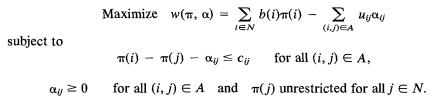
\includegraphics[scale = 0.75]{minimum_cost_flow_duality.png}
\label{fig: duality}
\end{figure}
\end{frame}

\begin{frame}{Minimum Cost Flow Duality}{Weak Duality Theorem}
\begin{block}{Theorem: }
  Let z(x) denote the objective function
  value of some feasible solution x of the minimum cost flow problem and let $w( \pi, \alpha)$
  denote the objective function value of some feasible solution $( \pi, \alpha)$ of its dual. Then
  $w( \pi, \alpha) \leq z(x)$.
\end{block}
\end{frame}

\begin{frame}{Minimum Cost Flow Duality}{Strong Duality Theorem}
\begin{block}{Theorem: }
  For any choice of problem data, the
  minimum cost flow problem always has a solution x* and the dual minimum cost
  flow problem has a solution $\pi$ satisfying the property that $z(x^*) = w(\pi)$.  
\end{block}
\begin{block}{Theorem: }
  If x is a feasible flow and $\pi$ is an (arbitrary) vector satisfying
  the property that $z(x) = w(\pi)$, then the pair $(x, \pi)$ satisfies the complementary
  slackness optimality conditions.  
\end{block}
\end{frame}

\begin{frame}{Minimum Cost Flow Duality}{Strong Duality Theorem (continue)}
\begin{block}{Theorem: }
  If $x^*$ is an optimal solution of the minimum cost flow problem, and $\pi$ is an optimal solution of the dual minimum cost flow problem, the pair
  $(x^*, \pi)$ satisfies the complementary slackness optimality conditions.
\end{block}
\begin{block}{Theorem: }
  Any linear program that contains (a) at most one + 1 and at most one -1 in each column, or (b) at most one + 1 and at most one -1 in each
  row, can be transformed into a minimum cost flow problem.  
\end{block}
\end{frame}

\begin{frame}{RELATING OPTIMAL FLOWS TO OPTIMAL NODE
  POTENTIALS}{Computing Optimal Node Potentials}
  The shortest path optimality conditions imply that
  \begin{equation}
    d(j) \leq d(i) + c_{ij}, \text{for all } (i,j) \in G(x^*) \label{ecuation}
  \end{equation}
  Let $\pi = -d$. Then we can restate \ref{ecuation} as: \begin{equation}
    c_{ij}^{\pi} = c_{ij} - \pi(i) + \pi(j) \geq 0, \text{for all } (i,j) \in G(x^*).
  \end{equation}  
\end{frame}

\begin{frame}{RELATING OPTIMAL FLOWS TO OPTIMAL NODE
  POTENTIALS}{Obtaining Optimal Flows} 
  Case 1: $c_{ij}^{\pi} > 0 $\\ 
  Implies that $x_{ij} $ must be zero. We enforce this constraint by setting $x_{ij}^*  = 0$ and deleting arc (i, j) from the network. \\ 
  Case 2: $c_{ij}^{\pi} < 0 $\\
  Implies $x_{ij}^* = u_{ij}$ We enforce this constraint by setting $x_{ij}^* = u_{ij}$ and deleting arc (i, j) from the network. Since we sent $u_{ij}$ units of flow on
  arc (i, j), we must decrease b(i) by $u_{ij}$ and increase b(j) by $u_{ij}$.
  Case 3: $c_{ij}^{\pi} = 0 $\\
  In this case we allow the flow on arc (i, j) to assume any value between 0 and $u_{ij}$.
\end{frame}

\begin{frame}{Algorithms}{CYCLE-CANCELING ALGORITHM AND THE
  INTEGRALITY PROPERTY}
\begin{figure}[h!t]
\centering
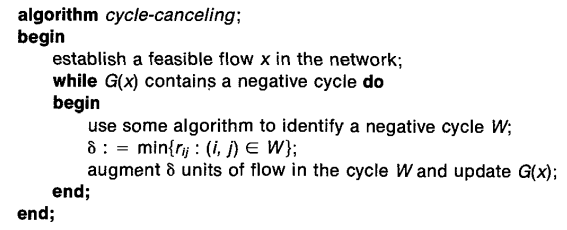
\includegraphics[scale = 0.6]{pseudocodigocyclecanceling.png}  
\end{figure}
\end{frame}

\begin{frame}{Algorithms}{CYCLE-CANCELING ALGORITHM AND THE
  INTEGRALITY PROPERTY}
\begin{figure}[h!t]
\centering
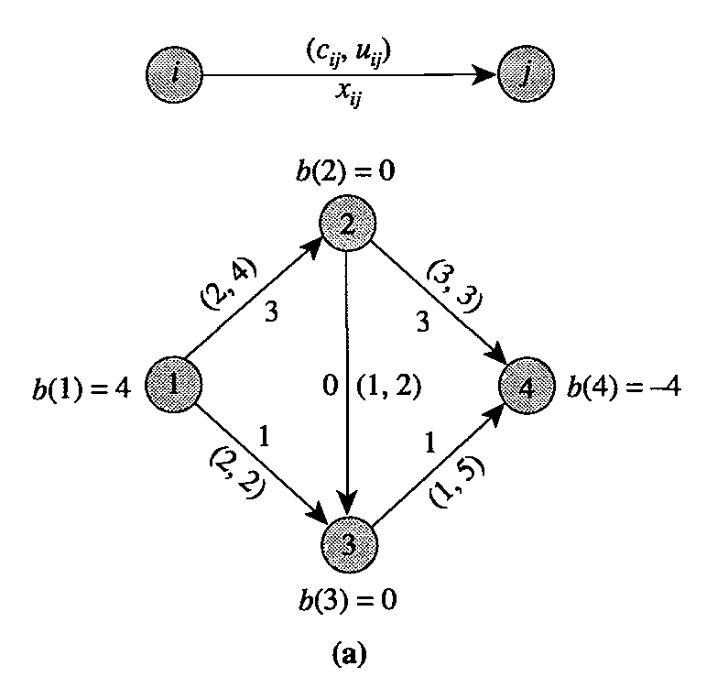
\includegraphics[scale = 0.25]{figura1cancelingcycle.png}
\end{figure}
\end{frame}

\begin{frame}{Algorithms}{CYCLE-CANCELING ALGORITHM AND THE
  INTEGRALITY PROPERTY}
  \begin{figure}[h!t]
    \centering
    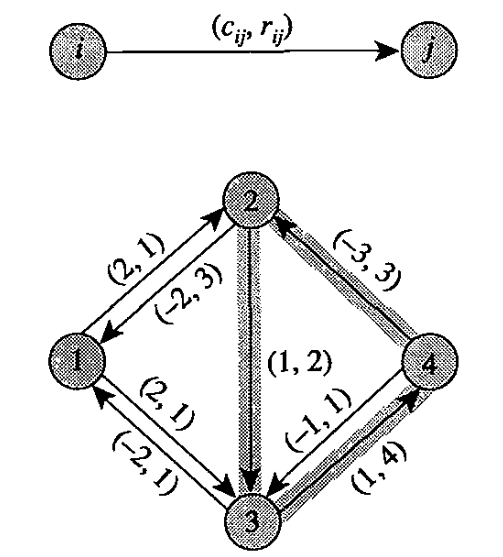
\includegraphics[scale = 0.3]{figura2canceling.png}
    \end{figure}
\end{frame}
\begin{frame}{Algorithms}{CYCLE-CANCELING ALGORITHM AND THE
  INTEGRALITY PROPERTY}
  \begin{figure}[h!t]
    \centering
    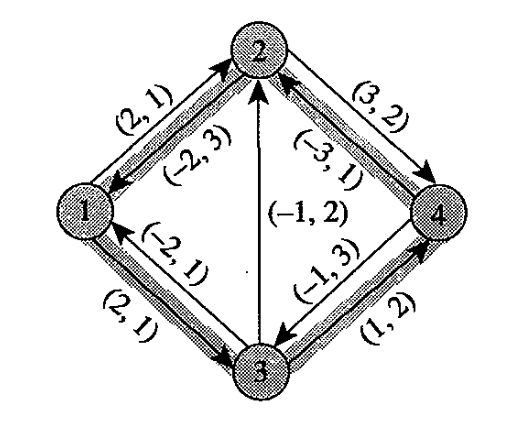
\includegraphics[scale = 0.4]{figura3canceling.png}
    \end{figure}
\end{frame}
\begin{frame}{Algorithms}{CYCLE-CANCELING ALGORITHM AND THE
  INTEGRALITY PROPERTY}
  \begin{figure}[h!t]
    \centering
    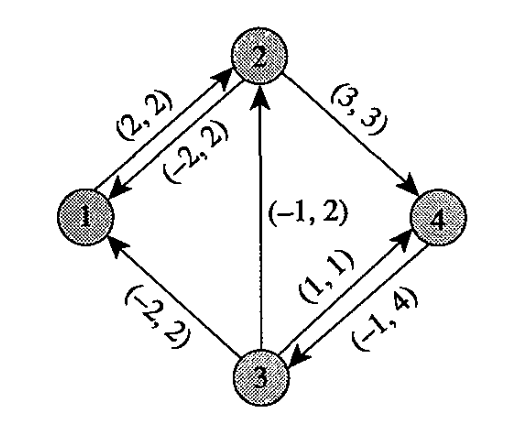
\includegraphics[scale = 0.4]{figura4canceling.png}
    \end{figure}
\end{frame}

\begin{frame}{Algorithms}{CYCLE-CANCELING ALGORITHM AND THE
  INTEGRALITY PROPERTY}
\begin{block}{Theorem: }
  If all arc capacities and supplies/demands
  of nodes are integer, the minimum costflow problem always has an integer minimum
  cost flow.  
\end{block}
\end{frame}

\begin{frame}{Algorithms}{SUCCESSIVE SHORTEST PATH ALGORITHM}
\begin{figure}[h!t]
\centering
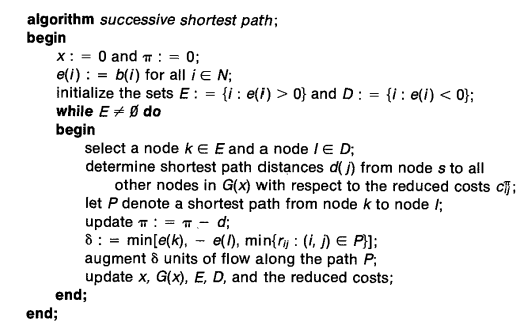
\includegraphics[scale = 0.55 ]{pseudocodigosuccesive.png}
%\caption{}
%\label{}
\end{figure}
\end{frame}

\begin{frame}{Algorithms}{SUCCESSIVE SHORTEST PATH ALGORITHM}
\begin{figure}[h!t]
\centering
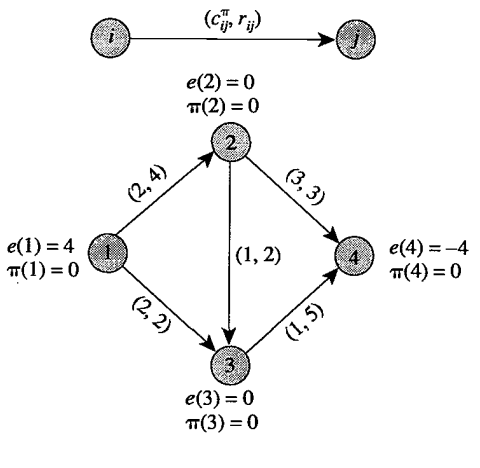
\includegraphics[scale = 0.4 ]{figura1succesive.png}
%\caption{}
%\label{}
\end{figure}
\end{frame}

\begin{frame}{Algorithms}{SUCCESSIVE SHORTEST PATH ALGORITHM}
\begin{figure}[h!t]
\centering
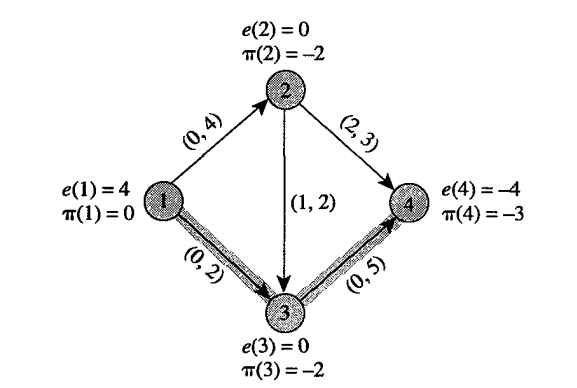
\includegraphics[scale = 0.5 ]{figura2succesive.png}
%\caption{}
%\label{}
\end{figure}
\end{frame}

\begin{frame}{Algorithms}{SUCCESSIVE SHORTEST PATH ALGORITHM}
\begin{figure}[h!t]
\centering
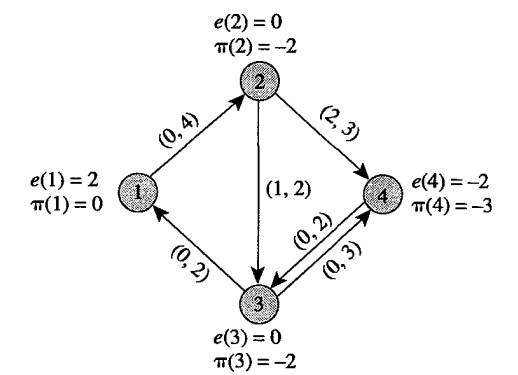
\includegraphics[scale = 0.5 ]{figura3succesive.png}
%\caption{}
%\label{}
\end{figure}
\end{frame}

\begin{frame}{Algorithms}{SUCCESSIVE SHORTEST PATH ALGORITHM}
\begin{figure}[h!t]
\centering
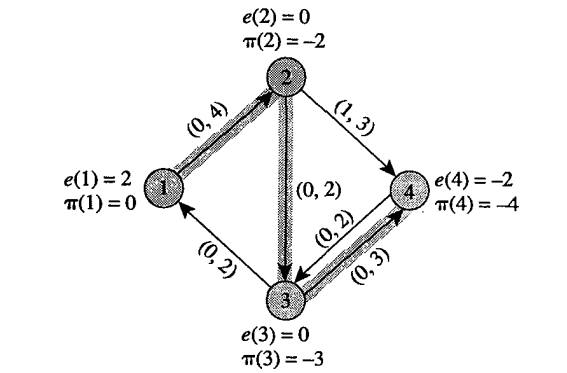
\includegraphics[scale = 0.5 ]{figura4succesive.png}
%\caption{}
%\label{}
\end{figure}
\end{frame}

\begin{frame}{Algorithms}{SUCCESSIVE SHORTEST PATH ALGORITHM}
\begin{figure}[h!t]
\centering
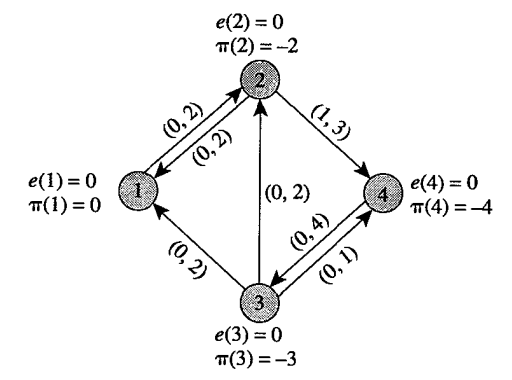
\includegraphics[scale = 0.5 ]{figra5succesive.png}
%\caption{}
%\label{}
\end{figure}
\end{frame}






\end{document}
